\documentclass[tikz,border=10pt]{standalone}
\usepackage{amsmath}
\usepackage{amssymb}

\begin{document}

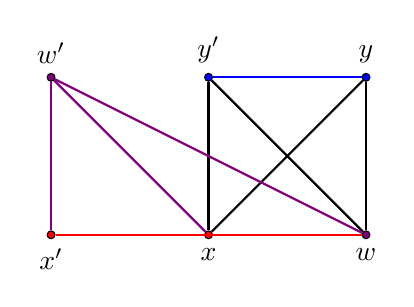
\begin{tikzpicture}[scale=2]

% Define points
\node[draw, circle, fill=red, inner sep=1pt, label=below:$x'$] (x') at (0,0) {};
\node[draw, circle, fill=red, inner sep=1pt, label=below:$x$] (x) at (1,0) {};
\node[draw, circle, fill=violet, inner sep=1pt, label=below:$w$] (w) at (2,0) {};
\node[draw, circle, fill=violet, inner sep=1pt, label=above:$w'$] (w') at (0,1) {};
\node[draw, circle, fill=blue, inner sep=1pt, label=above:$y'$] (y') at (1,1) {};
\node[draw, circle, fill=blue, inner sep=1pt, label=above:$y$] (y) at (2,1) {};

% Draw edges
\draw[thick, red] (x') -- (x);
\draw[thick, red] (x') -- (w);
\draw[thick, violet] (x') -- (w');
\draw[thick, violet] (x) -- (w');
\draw[thick, black] (x) -- (y');
\draw[thick, black] (x) -- (y);
\draw[thick, black] (w) -- (y');
\draw[thick, black] (w) -- (y);
\draw[thick, blue] (y') -- (y);
\draw[thick, violet] (w') -- (w);

\end{tikzpicture}

\end{document}